\chapter{阴雨}

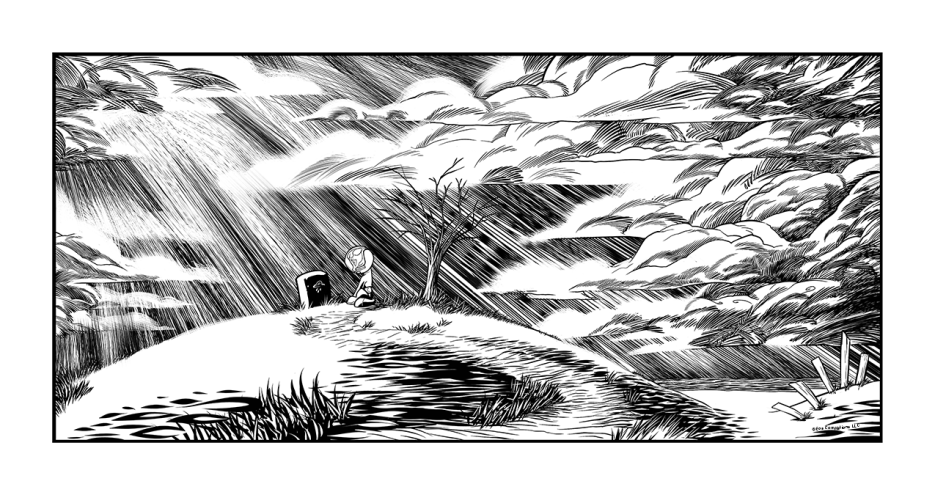
\includegraphics[width=0.9\linewidth]{image19.png}

\begin{intro}
    当风吹起时,摇篮就会摇摆,
    
    When the bough breaks, the cradle with fall,

    \medskip

    当树枝断裂,摇篮和宝宝会一起掉下来。\footnote{这一句是经典摇篮曲 \emph{Rock A Bye Baby} 睡吧宝贝的歌词}

    and down will come baby, cradle and all.
\end{intro}

\daytimeplace{14}{10:30 AM}{翡翠海岸,52号国道南段}{Emerald Shores, Big 52 S Branch}

帕比骑着滑板车在她的小跟班身边飞来飞去绕着圈子。

「耶……!你碰不到我!我超级快!」

尸鬼蹦蹦跳跳地想要跟上帕比,从远处看就好像两个穿着防辐射服的小孩子在嬉戏一样。不过或许这也是她们正在做的事情。一路玩耍让她们去翡翠海岸的旅程稍微慢了一点,不过这样也没什么关系。

「喏,跟班,」帕比停了下来,看着她的伙伴,「我不太确定妈妈喜不喜欢丑丑马,不过我会跟她说你是我的好朋友,而且你也找不到妈妈了,她肯定会帮你修好你的箭头……呃……不过,别做奇怪的事情好么,比如说马尾伯爵做的那种……呃……好么?我可不想第一天见妈妈就被关家门……」

那个生物歪着头,帕比把这个表情当做是肯定的回答,「那好,我来过这里好几次了,这里超超级好玩,只要你不问漂漂马太多问题就不会被妈妈训斥……问问题不是错,只是有些马不太喜欢某些谈话内容。」比如说,问为什么小马可以光屁股在大街上跑,但是为什么去海滩就必须穿比基尼之类的……帕比完全不知道为什么!

\horizonline

\daytimeplace{14}{11:00 AM}{铁砧镇,52号国道南段}{Ironworks, Big 52 S Branch}

砰……!砰……!

强盗的脑袋像个西瓜一样爆开了,在坏枪的掩护下,扳机熟练地给她的霰弹枪换着弹药。

「我们最好赶紧,乐乐,铁骑卫肯定也在附近清理……」

附近的爆炸把泥土溅了他们一头。

装好子弹之后,快乐扳机拉了一下枪栓,「没错,如果我们不想被多开几个洞的话。」雌驹说着飞奔到一座帐篷边,「掩护我破门。」坏枪移动到另一边的时候,雌驹冲进里面举起枪。

砰!砰!轰隆!

「咿!」

一堆电子设备炸成了五颜六色的火花和碎片。\thpr{打的好,乐乐,对于那些看起来像是机器的东西都是先打一枪再说。}这个帐篷里面有一张沙发,一堆箱子还有一台刚刚被她打爆的无线电……但是看起来里面一只小马也没有。

% TODO: 译文不合原文,此处改正

坏枪跟着走进来,「你愣什么呢?」

雌驹没有回答,警惕地看着周围,「我……我觉得刚刚好像听到一声惊呼……但是这里好像没有能发出惊呼的『漂漂马』。」

「那简单。」公马端起突击步枪,直接扫射了屋子一遍,在板条箱打了一排洞,打烂了小床,还把桌子上吃到一半的食物打成了一份现代派印象作品。然后他们听到了一声吃痛的惊叫,然后一个缩成一团的雌驹凭空出现在床底下,她肚子上的伤口留下一滩血。

「狗屎运……」乐乐喃喃自语,走进那个雌驹想一枪解除她的痛苦。她屁股后面有个白塔的可爱标记,那雌驹看起来那么年轻,一副失魂落魄的样子让卫兵迟疑起来。

「救救我……我还不想死……」独角兽闭着眼睛,在一阵阵剧痛带来的痉挛之间呻吟着,「妈妈……妈妈……救救我……」

「你等啥,她那样很痛苦的!」坏枪叹了口气走到那个雌驹身边举起枪。

「等等!」乐乐用蹄子推开公马的枪,她看着那个慢慢变得虚弱的雌驹,她还在祈求着她妈妈能来拯救她。

「我们……我们变成什么了?这个小马手无寸铁,只是躲在那里而已!」乐乐拿出一个治疗药水喂给她。

「你打算救活这家伙?为什么?她有机会绝对会毫不犹疑地杀了你!」坏枪不屑地打了一个响鼻,「而且她的『亲朋好友』说不定现在正在屠杀我们的盟友呢!」

乐乐回头白了那公马一眼,「你看到这个房间有任何武器么?」那个受伤的独角兽只剩下哭泣的力气了,不过乐乐还是给她喝了一些药水,「如果我们坚信,所有小马都是漂漂马,本性都是善良的,那么我们还是有机会重建昔日的小马国。」快乐扳机抱着小马要塞轻声唱着摇篮曲安慰着她。

坏枪坐在他的雌驹身边叹了口气,「你想太多了,总有一天会后悔。」

快乐扳机耸了耸肩继续唱。

\horizonline

\daytimeplace{14}{11:00 AM}{翡翠海岸,52号国道南段}{Emerald Shores, Big 52 S Branch}

帕比对面前的景象皱起了眉头,这里完全不是她记忆中的翡翠海岸!这里简直是一团糟,而且看不到一个马影!海边的所有小房子都变得脏兮兮的,而且海滩上也一片狼藉。

「怎么还没过多久这里就变成这样了?小马呢,音乐呢?婚礼庆祝呢?那些小店呢?还有……妈妈呢?」黄色的小雌驹伤心地低下了头,「抱歉,小跟班,看起来这里好像刚刚刮过台风。我想带你去玩旋转木马但是……」帕比回头用愧疚的眼神看着那个半腐烂的怪物,「我觉得现在那地方可能也没开门……」

那个尸鬼看起来毫不在意,但是帕比想给她的新朋友留下好的印象。

「哦,或许我们可以去看看糖果店好么?我们可以给妈妈准备个惊喜!」听起来是个不错的主意!给妈妈带上礼物一定能得到额外的抱抱和亲亲,「走,我们去商店血拼咯!」

小雌驹走下山丘,来到沿海的小镇上,小镇的建筑物都破旧不堪,窗户不是被打破了就是被木板钉上了,几乎城里的所有门都被木板封着。

「哇哦,刚刚过境的绝对是场大风暴!不过别担心,我知道有个买糖果的好地方!就在这个小巷子里面!」帕比一边说着,一边踩着小巷之中的水坑来到小路尽头。

「{\mt 警告,侦测到中等辐射,威胁等级:可忽略。}」

完全不管这个声音,小雌驹继续往前走着。

「{\mt 警告,侦测到大量辐射,威胁等级:可忽略。}」

帕比皱起眉头不爽地说:「喂喂,别胡说了,声音先生,拿出金币来!金闪闪的那种!我想要买好多好多糖果!」一堆金币浮到了小雌驹面前,她哼着歌转过拐角去找……

% NOTE: 补译一点

「这不公平!」

就在那个糖果店应该在的位置,现在是一个圆形的弹坑。帕比叹了口气,「好吧,好吧,别担心,我还知道很多可以买东西的地方。」不管怎么说,这里有很多很多小商店可以买好东西,怎么可能所有的商店都不见呢?

\horizonline

\daytimeplace{14}{11:15 AM}{铁砧镇,52号国道南段}{Ironworks, Big 52 S Branch}

白先生飘着一把来复枪从帐篷口探进头来。

「有谁受伤了?」

坏枪转头看着白苹果的老大说:「理论上是这样,刚刚我们打伤一个强盗,乐乐正给她急救呢。」

「哦,好吧,你们慢慢来,铁骑卫正在……等等,你说啥?」老白走进了帐篷看着那俩小马,「我们难道不就是来消灭他们的么?什么时候改变计划了?」

坏枪耸了耸肩,「你问他,好像和『漂漂马』啥的有关系。」

「闭嘴老枪,这个雌驹是非战斗成员!她只是带着隐形小马躲在床下而已,完全没有任何武器。我是个士兵,不是杀手。」快乐扳机一边说着一边用一个床单给雌驹盖好。

白先生摇了摇头,「我说,我们没时间搞这个了,野牛帮在撤退,我们必须立刻追击!我们没时间玩好马游戏了!我们越快结束这场战斗,就能越快在那个关于帕比的『阴影』什么预言落在我们头上之前赶过去。」

当听到帕比这个名字的时候,那个受伤的小马神经质地低语起来,「幽灵……是她在这个不洁之雾里召唤了不死同伴……她们是来吞噬你们的灵魂,是来杀死所有小马的!这都是我的错,我的错!为什么我要惹幽灵生气!妈妈……救命!」

「幽灵?不死?这只是个迷雾魔法而已,她在叨叨些什么?」白先生扬起了一边眉头。

坏枪清了清喉咙,「实际上,在来这里的路上,我们发现三个小马被……嗯……撕成了碎片。好像有谁用蹄子把他们给生撕了,那情景还真是挺可怕的。」

乐乐点点头,「没错,我们显然不是突袭这里的第一梯队……在我们之前,这里的小马已经在疯狂乱射了。」

白色的公马哼了一声,「真不错,这可以解释为什么还没等我们来这里就听见一堆枪声……不过现在有谁可以跟我解释她在念叨什么吗?」他戳了戳那个雌驹,「嘿,你能听到我说话么?你惹谁生气了?又是谁袭击你们了?」

「幽灵……52号国道的小幽灵……我们……不……是我……我打了她的屁股……她的泪水引来了恶魔……黄色幽灵……像她一样。但是……更残忍无情的不死怪物……她们杀了血浴……现在她们找我来了!是我打了她的屁股!是我打了屁股!全都是我的错!」

小马要塞歇斯底里地尖叫个不停,帐篷里面的三个小马一起用力才按住她。

「喂喂!冷静!这里没什么黄色恶魔!她们早走了,别挣扎,你还很虚弱!」坏枪终于坐在那个雌驹背上让她冷静下来。

「你……打了……帕比的……屁股?」白先生听到这里差点没忍住笑出来,「真的?我可是错过了最有趣的部分……」

\horizonline

\daytimeplace{14}{11:15 AM}{纪念碑镇,52号国道南段}{The Memorial, Big 52 S Branch}

「亲,你做得够好了。」

萍琪派坐在了长耳的身边。

先知长叹一声,从恍惚之中回过神来。

「我……好累……」

「亲,别担心,第一次都是这样的,不过你习惯这种感觉之后就好了。」

独角兽雌驹想要站起来,但是她的四条腿已经支撑不住自己的重量了。

「唉,到此为止了么?」

「还没……不过我觉得也没剩下多少了。亲你太过努力了,我早就警告过你,记得吗?」萍琪微笑起来,「不过别担心,一点痛苦都没有的,我们还可以一边等一边玩游戏!」

长耳露出一个虚弱的笑容,虽然死前还有个幻觉朋友可以聊天,不过在他乡异地因为毒品而孤独地死去,这个代价实在太高了——但是这一切都是有意义的。

「告诉我,她会一切平安么?」

「为什么问我?亲才是萨满哦!咱不过是个普通的漂漂马而已啦,哦,哦,你想要玩钉马尾游戏么?」

「求你了……我……我必须知道。」

叹了口气,萍琪皱起了眉头,「好吧,为啥大家全都这么无趣?好啦好啦,我说就是!她不会平安……至少现在不会,还需要最后一步,不过那个魔法迷雾相当不赖。」

独角兽虚弱地叹息,「那么,至少我死得还有价值……」

「亲,别皱眉都皱成梅干菜了!我们还要去准备派对呢!那个雾超级漂漂,把所有东西都掩盖了,帮了那些可怜的小幽灵一个大忙……至少你在最后一段旅程里给了那个小小幽灵一个可以陪伴她的朋友……不管怎么说,亲你逆转了命运!这绝对是值得庆祝的大喜事!呃……虽然把亲的小命搭上了,不过不管怎么说都应该高兴,不是么?」

……{}

「对吧?」

……{}

「哎,你看看她,又睡着了!好了!别睡了,起床了亲!我们该出发了,不然会迟到哦!」

\horizonline

\daytimeplace{14}{11:45 AM}{铁砧镇,52号国道南段}{Ironworks, Big 52 S Branch}

「你他妈跟老娘说什么?」赫瑞咆哮着,尖锐的喙几乎扎到了诘责的鼻尖,「什么叫『她不在这里』?」狮鹫完全不管其他铁骑卫对着她的枪口,继续对老书记官怒吼着。「你这个骗子!我信任你,干了你让我干的事情!现在你说她不见了?」

展开翅膀的狮鹫发出一声怒啸,对那掠食动物的吼叫毫不动容的诘责清了清喉咙,伸起蹄子示意那些铁骑卫放下枪。

「我知道我们曾经有过约定,不过她醒来以后自己跑掉了,你也知道那个孩子自个儿乱窜的时候想要让她呆在原地有多难,对吧?」

赫瑞塔眼底的岩浆似乎随时会喷发出来,「你知道现在她跑哪儿去了?」

诘责耸耸肩,「上一次见她的时候,她正往翡翠海岸去,不过我又不是先知……」

那佣兵面无表情地说:「我猜,她往南走了是吧。」

铁骑卫点点头,「就在海边,错不了。」

孤狼从旁观的马群里面走了出来,「等等,狮鹫,你想去那边的话,我和你一起去!」雄马展开翅膀跟上了赫瑞塔,「我觉得我们应该等等其他马,那里可能会有危险!」

「没错,等等,老娘等够了。在你们整个肏蛋奇蹄类动物里面,老娘只关心一位,而那位现在不在场……滚边儿去吧,小马!」赫瑞塔啐了一口,就好像要吐掉喙之中的恶心味道一样,然后张开翅膀消失在工厂屋顶之后。

「我现在就去追上她,你们尽快跟上我们好么。」

白先生以蹄覆面,「真是个好计划,先是单独行动,然后又是添油战术么,难道不是有什么南边的邪恶黑影啥的预言么?我们已经把我们那花里胡哨的专家丢在脑后了,现在又要分开行动。要我说,我们还是检查一下这里的生还者,然后决定怎么处理俘虏,最后等长耳来了一起往南走好么?」

「说到往南走……有谁看到融金了?」快乐扳机看着周围问。

天马嗤之以鼻,不耐烦地刨着地面,「这里有天杀的十五个铁骑卫!十五个!这群家伙绝对可以解决土匪的残兵败将,然后帮下面那些小马打开避难厩!现在我更关心那个幽灵而不是52号国道的地盘划分!我去追那狮鹫去了,你们最好也快点!这可不是个会等你们的派对,如果先知没错的话,我们时间不多了。」留下这几句话,孤狼飞走了。

\horizonline

\daytimeplace{14}{12:00 AM}{翡翠海岸,52号国道南段}{Emerald Shores, Big 52 S Branch}

帕比一点都不开心,她完全没找到任何给妈妈的礼物。或者说,她在整个城里连一只小马都没找到,这让她开始紧张起来。小雌驹觉得哪里不对劲,她开始担心妈妈会不会又跑到另一个地方去了。

所以她急忙冲向那个粉色箭头指向的海边小山丘,帕比在城里闲逛的时候,那个箭头一直没变过,不过帕比以前也遇到过这种事情,每一次旧的箭头消失就会有新的箭头出现,一次又一次地出现。

「好吧,小跟班,我们去找妈妈,或许这一次是对的!」

两个小孩子慢慢爬上泥泞的小小山路,这个山丘有一片微枯的黄绿色草坪,还有一颗死去很久的老树,帕比来到山顶的时候,她看到那里也有很多很多的小石头,每一块上都刻着一个名字和可爱标记,就像另一个爸爸的地方一样……好奇怪啊,为什么会有另一个爸爸的地方?

一只小马正坐在那颗只剩下枝干的树下,他慢慢站了起来,走向帕比和她的新朋友。

小雌驹飞奔向来者。

「妈咪!」

帕比的声音里充满了希望,但是很快又变小了。

「你……不是妈妈……」

在帕比身后的小跟班冲着来者发出了威胁的低吼声。

「不,帕比,我不是你的妈妈,抱歉……」融金用他那沙哑的声音说着,然后走到了一个布满苔藓的灰色石头面前,

「我真的……很抱歉……」

小雌驹走到了那个尸鬼身边,然后注意到那个粉色的箭头原来是指向这块石头的。虽然石头上的字迹早已经风化得模糊不清,不过她可以清楚地看到,那个一朵云和三点雨滴的可爱标记。

那是……妈妈的……可爱标记。

妈妈……{}

\horizonline

\daytimeplace{14}{12:00 AM}{翡翠海岸,52号国道南段}{Emerald Shores, Big 52 S Branch}

「好了,都安排好了。」白先生和诘责一起走了出来。

快乐扳机点点头。「好吧,那里一点都不远,我们别磨蹭了。」

诘责看着远处那个指示翡翠海岸方向的标志牌,只有六公里而已,天气好的时候都可以清楚看到小镇。

「如果那里情况不妙的话,我们要尽可能地拖延时间。」

「那还不赶紧!」快乐扳机说着沿着52大路开始向南边飞奔。

「好吧,谁最后到谁就是赤兔!」灌木笑着看了他叔叔和老书记官一眼,然后跟上那雌驹的速度。

诘责叹了口气,「这帮小年轻,他们绝对会在半路就累趴下的。」两个老公马跟着其他小马一起奔向海岸。

\horizonline

\daytimeplace{14}{12:10 AM}{翡翠海岸,52号国道南段}{Emerald Shores, Big 52 S Branch}

尸鬼什么也没说,只是静静地站在那里,让帕比有时间理解这个现实。

「妈妈……在这里?但是……」

小雌驹盯着这块石头,想要理解到底发生了什么,而跟班则坐在了头领身后。

「她……和爸爸……走了?但是……但是……不……不要……」帕比的声音越来越小,好像她声音太大的话,这个残酷的现实就无法改变一样。

「但是……我……我也想去……我……我想去见爸爸……为什么……为什么她把我留在家里?我……我……」

帕比失声痛哭起来。

「我真的没有不听话……我只是……我只是想要看烟火!我……我不知道我的房子会倒掉我妈妈会走掉……我……我……」帕比一屁股坐在了地上,低头看着自己的蹄子。

「只是想看那个破烟花而已……为什么接下来一切都一团糟!我很抱歉……我错了……我真的错了……对不起……妈妈……请回来呀!」

帕比嚎啕大哭,绝望地对着那块埋葬着她母亲的墓碑大声哭道:「妈妈!你……你说什么我都听!训我吧!打我吧!但是别扔下我啊!」

融金看着他面前的可怜生灵,想要说些什么,说任何事情,但是这一幕实在太过悲哀,让他说不出一个字。而这个时候,她抬起了头,于是那双泪流不止的双眸和他对上了。

「求求您,求求您告诉我妈妈去哪儿了!我把我的玩具给您好吗,我愿意把我所有东西都给您,好吗?还是您想要更多漂漂玻璃珠?我会为您把所有的玻璃珠都找到,好吗!求求您!求求您了!」帕比站起来走向那个老尸鬼,而小雌驹沉重的视线让他不由得后退了几步。

「帕比……我很抱歉,但是……这里就是你妈妈长眠的地方……她……已经死了……她很久很久之前就已经去世了。」

帕比笑了,但是那微笑毛骨悚然。那双空洞的眸子盯着融金,不住地颤抖着,「死了?只是死了?她死了?那没关系的!她会好起来的吧!我也已经死了,但是你看我很好啊!你也死了但是你也很好啊!死了没什么不好的对吧?我们只要在这里等就好了,对吧?对吧?对吧!」

融金看着那天真的小孩子,死了……还会好起来?只要在这里等?

「帕比……不是这样的……她……她已经不会回来了……她已经去世了……她已经……帕比……你可以跟我在一起,好么?我永远不会丢下你。虽然我不是你妈妈……」

「怎么有俩帕比?到底发生什么了?」赫瑞塔一个猛地降落在地上,压坏了好几根树枝。「僵尸,把你的脏蹄子从我朋友身上拿开!」狮鹫落在融金和帕比之间举起枪指着尸鬼。

黄色的小雌驹很快就认出了新来的狮鹫,「赫瑞!赫瑞!妈妈……妈妈……妈妈她……妈妈她不要我了……她和爸爸走了……丢下我不会回来了……我……我我……帮帮我!」

佣兵看了看那个用蹄子指着墓碑的尸鬼,然后明白了帕比在说什么。

「肏你妈,老娘……来迟了……」

赫瑞塔转身用一只爪子抚摸着帕比的头盔,「帕比,我会陪你,好吗?你不会孤独的。」

「但是……我想我妈妈!我要我妈妈!她……只有她才能……只有她才能把一切都修好!她可以修好坏掉的房子,修好这个破太空服,找到跟班的妈妈,让之前快乐的日子再回来!没……没有她我都不知道该怎么办!」

什么也没说,狮鹫紧紧地抱住了帕比。

「但是……但是你自己就已经做的很好了,帕比……你救了我,你还救了整个太阳城!你还阻止了铁骑卫的内战!你还……你……你是个好孩子!你是我认识的唯一一只好小马!不需要你妈妈,你就可以解决一切。让我当你的姐姐,好么?赫瑞和帕比,最佳组合!」

「狮鹫说的没错,帕比……你已经长大了,你妈妈会为你自豪的。」

帕比挣扎着推开了赫瑞塔,她的双眸之中燃烧着粉色的火焰,「但是她把我丢在这里!她扔下我和爸爸一起走了!我那么爱她,为什么她要扔掉我?为什么她不爱我?」

「你丫到底想……」赫瑞塔摇了摇头,「你到底说什么呢?她没有选择扔下你,她只是迫不得已。她绝对不会丢下你不管,她以为你在避难厩里面会平平安安的长大,否则她绝对不会把你丢在这么危险的地方的!」

孤狼落了下来,「呃……我不知道发生了什么,但是我觉得对小孩子大喊大叫没什么用。」

「我说也是,狮鹫小姐,所以我一直不……」

帕比打断了那两个公马的碎碎念,大声吼着:「那么为什么她不回来接我一起去?」

「傻瓜,她已经死了!死了!懂不懂!」赫瑞塔锋利的喙顶着帕比的头盔,和小雌驹对视着,融金想拉开狮鹫,但是小跟班低吼着拦住了他。「妈妈不会再回来了!你已经永远失去她了!这就是命运!她现在就躺在这个坟墓里面,绝对!再也!!不会!!!回来了!!!!所以你要坚强起来,将你自己的命运踩在蹄下!别管那破墓碑了,现在就跟我走!」

狮鹫转头看着那个老木乃伊和天马,不过她马上注意到一大堆小马正在从北边赶来。

「看到没有?你的朋友来接你了!你让大家都担心坏了,别再这样失落了,伸出蹄子站起来好么!」

帕比看了看过来的马群,然后又看了看那个有可爱标记的墓碑。

「妈妈……在这里面?」

赫瑞塔完全没有注意到帕比的表情和融金拼命的示意,只是说着自己的话,

「没错,你妈永远都躺在这里,你什么时候想来看她都可以,现在跟我来,一起和你的朋友说你一切安好,好么?」

「石头!」

帕比尖叫着举起了「命运之石」,然后用力砸向那个墓碑。

「你丫在干什么?」赫瑞塔想阻止她的朋友,但是小跟班跳到了她们俩之间,即使是勇敢的狮鹫也被那双红色的眼睛吓住了。

「妈妈,妈妈出来啊!」帕比用她所有的力气砸着墓碑,融金和孤狼被这碎石飞溅的景象吓坏了。

「等等孩子!那样她也不会回来的!别这样,你会……你会打坏你妈妈的坟墓的!」孤狼跳了起来落在石头边挡住了帕比的蹄子。

「你到底怎么了?别这样!」

「放开……放开我……放开我!我想要妈妈!为什么妈妈不见了!」

跟班转头吼着天马的时候,赫瑞塔立刻冲过来打上帕比的头。

「傻瓜!给老娘振作起来啊!丫的真想打你的屁股!忘了你妈妈吧,傻瓜!你现在和我在一起了,别想不可能的事情,醒醒吧!」

被狮鹫的愤怒搞迷糊的帕比愣住了,小雌驹慢慢地转向大海,「但是……但是……我把她忘掉的话……我找不到妈妈的话……我……还能做什么呢?」

赫瑞挥着爪子说:「那我们就一起去找些快乐的事情来做,好么?你冷静下来,我会替你想办法的!乖乖的……乖乖的坐好……你看,你的朋友都在这里。」

老白,诘责,快乐扳机和坏枪正跑向山丘,虽然他们看起来精疲力竭,但是诘责还是喘着粗气问。

「发……发生什么了?」

帕比看了一眼蹄子中的「命运之石」,低声说:「我……我不想醒来……我只想……永远睡下去……再也不醒来……」

赫瑞塔拍着帕比的头盔微笑着:「我知道那种感觉……但是,总有一天会消失的,你也一样……乖乖坐在这里冷静一下,我们去招呼新来的小马,好么?」

黄色的小雌驹虚弱地点了点头,「命运之石」第一次从她蹄中滑落,滚下山丘,在山坡上来回弹了几下,最后随着一声金属敲击声落在了海滩上。

\horizonline

\daytimeplace{14}{12:25 AM}{翡翠海岸,52号国道南段}{Emerald Shores, Big 52 S Branch}

融金和孤狼已经走向了新来的马群,赫瑞塔也走了过去,把帕比和她的黄色小伙伴孤零零地留在坟墓边。

「别担心,她会好起来的,她现在只是需要独处一会儿。」

「但是……她在哭么?她怎么样了?」

帕比觉得如此……空虚。不是悲伤,也不是愤怒,也不是她以前感觉到的任何感情。她就在她妈妈面前,但是妈妈却不在这里,再也不会抱着她,对她微笑了……{}

「……虽然我不是那么多心,但是我还是想看看她的情况……」

「……那小心另一个尸鬼,那东西看起来蛮凶的……」

大家都在乱糟糟地说着什么,在帕比听来就是一阵嗡嗡的声音。帕比不关心,她只是慢慢地沉浸下去,慢慢地沉入内心深处。

再也见不到妈妈了。这个想法已经让她失去了所有力气,她顺着这条路走了这么远,唯一的目的就是想要再见到她的妈妈,但是现在什么也没有了。她很喜欢她的朋友,但是她觉得这样不对,这里根本不是她应该在的地方,她根本就不想呆在这种地方!或许……或许会有什么地方……不一样的地方……更好的地方……{}

「……那么就是这样了?我们做到了?52号国道安全了?那孩子也没事了?好了,我们现在回家吧……」

回家……家又在哪里?家已经没有了,她在中心城的家已经没有了,妈妈已经没有了,再也回不来了,再也见不到她了。帕比不想这样活着,她不想要这样……每一天晚上都醒着,直到凌明的曙光再一次提醒她又是没有妈妈陪伴的一天……她不想醒来,只想就这样睡去。

\pypr{「哦,那很简单,小家伙,你只要和我许个愿,我就会让你静静地睡去,做一个永远永远不会醒来的美梦。」}

「……闭嘴老枪!我们离开几天而已,隧道镇又不会烧了!」

「真的?你能做到么?」

\pypr{「那当然!我可是梦之主,我可以给你所有的快乐,你只要向我许个愿。」}

「……野牛帮还没完,我们只是把他们赶走而已,但是我觉得我们应该想出一个和平解决方案……」

「……我不觉得他们会同意的,老爸,野牛帮可不吃爱与宽容那一套……」

「……或许现在他们的王牌都打光了,他们会更……讲理……诘责,我觉得我们至少应该试试看……」

「永远永远的永远?」

\pypr{「比永远还要更长久,这是你我之间的约定哦。我可以让你在梦中和你爸爸妈妈永远过着幸福快乐的生活,而你嘛,只要让我在你睡着之后做一点点小事就好啦,可不可以啊?」}

小跟班尖叫着拼命戳着融金的后背,但是大家似乎全都更加专注于老白和诘责之间关于52号国道将来格局的讨论,没有注意那个小小的中心城尸鬼。

「我在52号国道混了这么多年了,我记得野牛帮最早可不是那么凶恶,他们只是52号国道上的游牧民,只是因为52号国道的每个居民点都对他们课以重税,但野牛帮在重税之下买不起任何他们想要的补给,所以他们才铤而走险……如果每一个族群都友善那么一点,也不会落得如此结果。」

「……我可不那么想……我祖父总是说野牛帮一直在找机会咬你一口……」

% TODO: 如何修正这里?

「……第一个对野牛帮课税的就是老白你祖父!你难道一点想要改变这个的常识都没有么?」

一声悠长的叹息,帕比点点头,「好的,就那么做吧!」

\pypr{「你的选择很正确,你绝对不会后悔的。」}

「做什么啊,帕比,我虽然很喜欢你,但是废除马头税可没那么简单,大人说话小孩子别插嘴好么!」

「对,没错,请……让这一切都消失吧。」

\pypr{「我真是太喜欢你的天真纯洁了……我会想念你的,来吧,请闭上你的眼睛……」}

~\vfill

\begin{note}
    升级(Lv 18)

    新技能解锁:就是现在!——你立即升一级。

\end{note}

\begin{note}
    升级(Lv 19)

    新技能解锁:专注射击——在S.A.T.S.状态下,你瞄准对手的特别部位时得到5\%的命中率加成……你想说啥,帕比已经绝望到开始胡乱选专长了,她根本没有S.A.T.S.!

    新任务专长解锁:移动梦魇(等级3)——耶!你现在就是梦魇了!不过这对你的社交生活没什么好处,因为你对所有派系的声望都变成了敌视。至于属性奖励就不在这里写了,因为太长写不下了。
\end{note}


